\documentclass[journal,10pt]{IEEEtran}
\usepackage{sharina}

\begin{document}
\onecolumn
\subsection{Easy}

\begin{table}[htbp]
    \centering
    \caption{No. 1 in Easy Set}
    \label{tab:easy1}
    \begin{tabular}{|l|c|p{5cm}|p{5cm}|} 
    \toprule
    \multicolumn{1}{|c|}{\multirow{2}{*}{Image}} & \multirow{2}{*}{Models} & \multicolumn{1}{c|}{QA 1}                                                            & \multicolumn{1}{c|}{QA 2}  \\ 
    \cline{3-4}
    \multicolumn{1}{|c|}{}                       &                         & Can you describe the spatial relationship between the cat and the white remote control? & Is this answer correct?    \\ 
    \hline
    \multirow{3}{*}{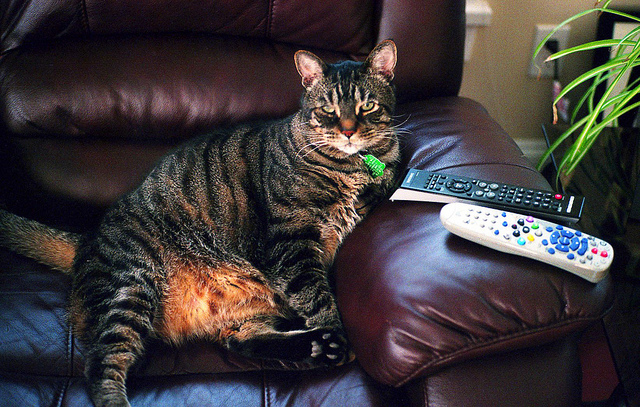
\includegraphics[width=0.25\linewidth]{../image set/easy/000000000599.jpg}}                            & GPT-4+ SenceXplain      &                                                                                      &                            \\ 
    \cline{2-4}
                                                 & Bard                    &      
                                                 
Sure. The image you linked to shows a cat sitting on a couch. The white remote control is on the couch next to the cat. The remote control is slightly in front of the cat, and it is to the cat's right. The remote control is also slightly higher than the cat, as it is resting on the armrest of the couch.

Here is a more detailed description of the spatial relationship between the cat and the white remote control:

The cat is sitting on the couch, and the remote control is on the couch next to the cat.
The remote control is slightly in front of the cat, and it is to the cat's right.
The remote control is also slightly higher than the cat, as it is resting on the armrest of the couch.
The cat is facing the remote control, and the remote control is facing the cat.
The cat is slightly obscuring the remote control, but the remote control is still visible.
I hope this helps!                                                                              &   
Yes, your answer is correct. You have described the spatial relationship between the cat and the white remote control in a clear and concise way. You have also identified some of the more specific details of the relationship, such as the fact that the remote control is slightly in front of the cat and to the cat's right. Additionally, you have mentioned the way in which the cat is slightly obscuring the remote control, but the remote control is still visible.

Overall, your answer is very good. It is clear, concise, and accurate. You have clearly understood the spatial relationships between the cat and the white remote control in the image and you have been able to describe them in a way that is easy to understand.

I hope this helps!                         \\ 
    \cline{2-4}
                                                 & Visual ChatGPT          &                                                                                      &                            \\
    \bottomrule
    \end{tabular}
\end{table}
\end{document}